\documentclass{standalone}
\usepackage{tikz}
\usetikzlibrary{arrows,positioning,decorations.pathreplacing} 
\tikzset{
    %Define standard arrow tip
    >=stealth',
    %Define style for boxes
    point/.style={
           rectangle,
           rounded corners,
           draw=black, very thick,
           text width=5em,
           minimum height=2em,
           font=\sffamily,
           text centered},
    annote/.style={
          font=\sffamily
    },
    % Define arrow style
    arrow/.style={
           ->,
           thick,
           shorten <=2pt,
           shorten >=2pt,},   
}

\begin{document}
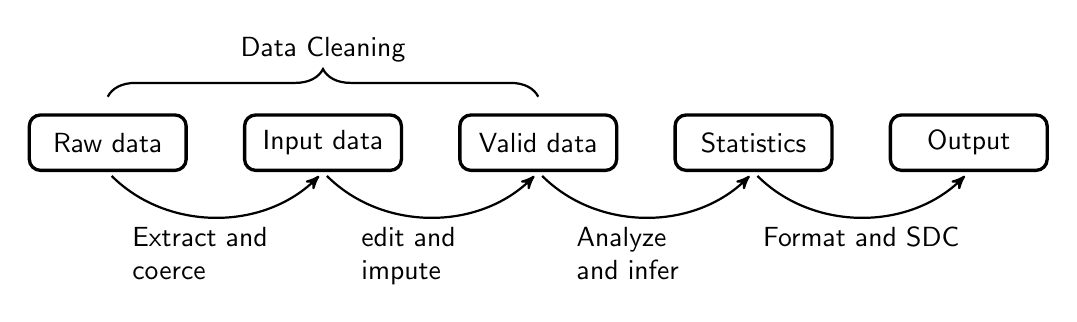
\begin{tikzpicture}
\node[point]                          (raw) {Raw data};
\node[point, right=7mm of raw]        (tech){Input data};
\node[point, right=7mm of tech]       (consistent){Valid data};
\node[point, right=7mm of consistent] (estimate){Statistics};
\node[point, right=7mm of estimate] (output){Output};
\path (raw.south) edge[arrow, bend right=45] node[below,annote,text width=6em] {Extract and coerce} (tech.south);
\path (tech.south) edge[arrow, bend right=45] node[below,annote, text width=5em] {edit and impute} (consistent.south);
\path (consistent.south) edge[arrow, bend right=45] node[below,annote, text width=5em]  {Analyze and infer} (estimate.south);
\path (estimate.south) edge[arrow, bend right=45] node[below,annote] {Format and SDC} (output.south);
\path (raw.north) edge[decorate,decoration={brace,raise=6pt,amplitude=10pt}, thick]
     node[above=15pt,annote]{Data Cleaning}  (consistent.north) ;
\end{tikzpicture}

\end{document}
